\chapter{Phân tích yêu cầu}
\section{Phân tích yêu cầu nghiệp vụ}
\subsection{Yêu cầu chức năng}
\noindent Hệ thống có một số tính năng chính sau:
\begin {list} {-}{}
    \item Người dùng có thể đăng ký tài khoản cho riêng mình.
    \item Người dùng có thể đăng nhập vào hệ thống với tài khoản và mật khẩu đã đăng ký thành công trước đó.
    \item Người dùng có thể đổi mật khẩu khi cần thiết.
    \item Khi truy cập và hệ thống, người dùng có thể xem được tất cả các sản phẩm của cửa hàng.
    \item Hệ thống có thể phân loại sản phẩm theo từng loại khác nhau.
    \item Người dùng có thể tìm kiếm sản phẩm theo tên, loại, giá, kích thước\dots
    \item Người dùng có thể xem chi tiết sản phẩm để lựa chọn được sản phẩm phù hợp nhất.
    \item Người dùng có thể thêm sản phẩm vào giỏ hàng.
    \item Người dùng có thể xem giỏ hàng của mình.
    \item Người dùng có thể xóa sản phẩm, điều chỉnh số lượng sản phẩm trong giỏ hàng.
    \item Người dùng có thể xem tổng số tiền hiện tại của giỏ hàng.
    \item Người dùng có thể thanh toán những sản phẩm trong giỏ hàng bằng nhiều hình thức khác nhau như: tiền mặt, thẻ tín dụng, ví điện tử\dots
    \item Người dùng có thể xem lịch sử mua hàng của mình.
    \item Người dùng có thể để lại những đánh giá về sản phẩm mà mình đã mua.
    \item Hệ thống phân quyền người dùng theo từng vai trò khác nhau gồm có: khách hàng (customer), nhân viên (staff), quản lý (manager).
    \item Khi đăng nhập với vai trò là nhân viên, người dùng có thể thêm, sửa, xóa, điều chỉnh sản phẩm và quản lý đơn hàng.
    \item Khi đăng nhập với vai trò là quản lý, người dùng có thể thêm, sửa, xóa, điều chỉnh sản phẩm, quản lý đơn hàng, và quản lý người dùng sử dụng hệ thống (thêm, sửa, xóa, chặn\dots).
    \item Hệ thống thống kê doanh thu thành biểu đồ theo từng ngày,tháng,năm để nhân viên và quản lý có thể dễ dàng theo dõi.
\end {list}
\subsection{Yêu cầu phi chức năng}
\noindent Hệ thống có một số yêu cầu phi chức năng như sau:
\begin {list} {-}{}
    \item Hệ thống có giao diện thân thiện với người dùng.
    \item Hệ thống có thể dễ dàng sử dụng đối với người dùng mới.
    \item Hệ thống có thể hoạt động tốt trên hầu hết các trình duyệt hiện nay như Chrome, Firefox, Safari, Microsoft Edge\dots
    \item Hệ thống hoạt động tốt trên nhiều loại thiết bị khác nhau như máy tính, điện thoại, máy tính bảng\dots
    \item Hệ thống có thể chạy mượt mà, ổn định.
    \item Hệ thống có thể chịu tải tốt, phục vụ nhiều người dùng cùng một lúc.
    \item Hệ thống phục vụ người dùng 24/7.
    \item Hệ thống có thể bảo mật thông tin người dùng bằng những phương pháp mã hoá thông tin nhạy cảm.
\newpage
\section{Phân tích hệ thống}
\subsection{Use case diagram}
\subsubsection{Use case diagram cho toàn bộ tính năng của hệ thống}
\begin{figure}[H]
    \begin{center}
    \includegraphics[scale=0.45]{images/hieu/chap-3/usecase-diagram.png}
    \vspace*{5mm}
    \caption{Use case diagram cho toàn bộ tính năng của hệ thống}
    \end{center}
\end{figure}
\newpage
\subsubsection{Đặc tả use case cho một số tính năng chính}
\begin{itemize}
    \item \textbf{Đăng nhập}
    \begin{table}[H]
        \begin{tabular}{|l|l|}
        \hline
        \textbf{Use-case name}    & \textbf{Đăng nhập - Login}                                                                                                                                                                                                                                                                                                                                                                                                                           \\ \hline
        \textbf{Actor}            & User (Manager, Customer, Staff)                                                                                                                                                                                                                                                                                                                                                                                                                      \\ \hline
        \textbf{Description}      & Người dùng đăng nhập vào hệ thống                                                                                                                                                                                                                                                                                                                                                                                                                    \\ \hline
        \textbf{Pre-condition}    & Người dùng đã đăng ký tài khoản thàng công                                                                                                                                                                                                                                                                                                                                                                                                           \\ \hline
        \textbf{Post-condition}   & Người dùng đăng nhập thành công                                                                                                                                                                                                                                                                                                                                                                                                                      \\ \hline
        \textbf{Normal-flow}      & \begin{tabular}[c]{@{}l@{}}1.Người dùng chọn biểu tượng đăng nhập trên góc phải màn hình.\\ 2.Hệ thống hiển thị trang đăng nhập.\\ 3.Người dùng nhập thông tin đã đăng ký gồm tên người dùng (username) và \\ mật khẩu (password)\\ 4.Người dùng chọn nút "ĐĂNG NHẬP".\\ 5.1.Hệ thống chuyển đến "TRANG CHỦ" nếu xác thực thông tin thành công.\\ 5.2.Nếu thông tin sai, hệ thống yêu cầu người dùng nhập lại.\\ 6.Đăng nhập thành công\end{tabular} \\ \hline
        \textbf{Alternative-flow} & Không có                                                                                                                                                                                                                                                                                                                                                                                                                                             \\ \hline
        \textbf{Exception}        & \begin{tabular}[c]{@{}l@{}}Nếu người dùng bị chặn bởi người quản lý (Manager) sẽ không thể đăng nhập \\ vào hệ thống\end{tabular}                                                                                                                                                                                                                                                                                                                    \\ \hline
        \end{tabular}
        \begin{center}
            % Bảng 3.1: 
        \end{center}
    \caption{Đặc tả use case đăng nhập}
    \label{table:login}
    \end{table}
        
    \item \textbf{Đăng ký}
    \begin{table}[H]
        \begin{tabular}{|l|l|}
        \hline
        \textbf{Use-case name}    & \textbf{Đăng ký - SignUp}                                                                                                                                                                                                                                                                                                                                                                                                                                                                                                                              \\ \hline
        \textbf{Actor}            & User (Manager, Customer, Staff)                                                                                                                                                                                                                                                                                                                                                                                                                                                                                                                        \\ \hline
        \textbf{Description}      & Người dùng đăng ký tài khoản để truy cập vào hệ thống                                                                                                                                                                                                                                                                                                                                                                                                                                                                                                  \\ \hline
        \textbf{Pre-condition}    & Người dùng truy cập vào website thành công                                                                                                                                                                                                                                                                                                                                                                                                                                                                                                             \\ \hline
        \textbf{Post-condition}   & Người dùng đăng ký tài khoản thành công                                                                                                                                                                                                                                                                                                                                                                                                                                                                                                                \\ \hline
        \textbf{Normal-flow}      & \begin{tabular}[c]{@{}l@{}}1.Người dùng chọn biểu tượng đăng nhập trên góc phải màn hình.\\ 2.Hệ thống hiển thị trang đăng nhập.\\ 3.Người dùng nhấn vào liên kết "Bạn chưa có tài khoản?" \\ 4.Hệ thống chuyển sang trang đăng ký tài khoản.\\ 5.Người dùng nhập đầy đủ thông tin mà hệ thống yêu cầu như họ tên, email,\\ địa chỉ, số điện thoại...\\ 6.Chọn nút "ĐĂNG KÝ"\\ 7.1.Hệ thống hiển thị đăng ký thành công \\ 7.2.Hệ thống yêu cầu nhập lại thông tin nếu có sai sót (thiếu trường thông tin,\\ email không thể xác thực...) \\8.Hệ thống lưu thông tin người dùng.\end{tabular} \\ \hline
        \textbf{Alternative-flow} & Không có                                                                                                                                                                                                                                                                                                                                                                                                                                                                                                                                               \\ \hline
        \textbf{Exception}        & Một địa chỉ email chỉ đăng ký được một tài khoản.                                                                                                                                                                                                                                                                                                                                                                                                                                                                                                      \\ \hline
        \end{tabular}
        \begin{center}
        \end{center}
        \caption{Đặc tả use case đăng ký tài khoản}
        \label{table:signup}
    \end{table}
    \newpage
    \item \textbf{Xem sản phẩm}
    \begin{table}[H]
        \begin{tabular}{|l|l|}
        \hline
        \textbf{Use-case name}    & \textbf{Xem sản phẩm - View Products}                                                                                                                                                                                                                                                                                                                                                                                                                                                                                                                                                                                                                                                                                                                                                                           \\ \hline
        \textbf{Actor}            & User (Manager, Customer, Staff)                                                                                                                                                                                                                                                                                                                                                                                                                                                                                                                                                                                                                                                                                                                                                                                 \\ \hline
        \textbf{Description}      & Người dùng xem những sản phẩm được bày bán trên cửa hàng                                                                                                                                                                                                                                                                                                                                                                                                                                                                                                                                                                                                                                                                                                                                                        \\ \hline
        \textbf{Pre-condition}    & Người dùng đăng nhập vào hệ thống thành công                                                                                                                                                                                                                                                                                                                                                                                                                                                                                                                                                                                                                                                                                                                                                                     \\ \hline
        \textbf{Post-condition}   & Người dùng có thể xem sản phẩm của cửa hàng                                                                                                                                                                                                                                                                                                                                                                                                                                                                                                                                                                                                                                                                                                                                                                     \\ \hline
        \textbf{Normal-flow}      & \begin{tabular}[c]{@{}l@{}}1.Người dùng truy cập vào website.\\ 2.Hệ thống tự động chuyển đến trang chủ (HomePage).\\ 3.Tại trang chủ, người dùng có thể lướt để xem tất cả những sản phẩm được   \\ hiển thị theo loại, ngoài ra còn có những sản phẩm nổi bật, những sản phẩm\\ sắp được ra mắt trong tương lai.\\ 4.Người dùng có thể tìm kiếm sản phẩm mình muốn bằng cách nhập từ khoá \\ (tên, loại, giá, kích thước...) vào ô tìm kiếm rồi nhấn nút "TÌM KIẾM".\\ 5.Hệ thống hiển thị kết quả tìm kiếm.\\ 6.Người dùng nhấn vào từng sản phẩm \\ 7.Hệ thống hiển thị thông tin chi tiết của sản phẩm tương ứng.\\ 8.Nếu người dùng muốn mua sản phẩm:\\       8.1.Nhấn vào nút "MUA HÀNG" để trực tiếp mua sản phẩm.\\       8.2.Nhấn vào biểu tưởng giỏ hàng để thêm sản phẩm vào giỏ hàng.\end{tabular} \\ \hline
        \textbf{Alternative-flow} & Không có                                                                                                                                                                                                                                                                                                                                                                                                                                                                                                                                                                                                                                                                                                                                                                                                        \\ \hline
        \textbf{Exception}        & Người dùng phải đăng nhập mới có thể mua hàng hoặc thêm vào giỏ hàng.                                                                                                                                                                                                                                                                                                                                                                                                                                                                                                                                                                                                                                                                                                                                                                                                        \\ \hline
        \end{tabular}
        \begin{center}
        \end{center}
        \caption{Đặc tả use case xem sản phẩm}
        \label{table:product}
        \end{table}
        
        \item \textbf{Quản lý giỏ hàng}
        \begin{table}[H]
            \begin{tabular}{|l|l|}
            \hline
            \textbf{Use-case name}    & \textbf{Quản lý giỏ hàng - Cart Manager}                                                                                                                                                                                                                                 \\ \hline
            \textbf{Actor}            & User (Manager, Customer, Staff)                                                                                                                                                                                                                                          \\ \hline
            \textbf{Description}      & Người dùng quản lý giỏ hàng của mình                                                                                                                                                                                                                                     \\ \hline
            \textbf{Pre-condition}    & Người dùng đăng nhập vào hệ thống thành công                                                                                                                                                                                                                             \\ \hline
            \textbf{Post-condition}   & Người dùng quản lý giỏ hàng thành công                                                                                                                                                                                                                                   \\ \hline
            \textbf{Normal-flow}      & \begin{tabular}[c]{@{}l@{}}1.Người dùng nhấn vào biểu tượng giỏ hàng nằm trên thanh điều hướng.\\ 2.Hệ thống hiển thị chi tiết trang giỏ hàng.\\ 3.Tại đây, người dùng có thể.\\ -Thêm / Xoá sản phẩm khỏi giỏ hàng.\\ -Tăng / Giảm số lượng từng sản phẩm.\end{tabular} \\ \hline
            \textbf{Alternative-flow} & Không có                                                                                                                                                                                                                                                                 \\ \hline
            \textbf{Exception}        & Không có                                                                                                                                                                                                                                                                 \\ \hline
            \end{tabular}
            \begin{center}
            \end{center}
            \caption{Đặc tả use case quản lý giỏ hàng}
            \label{table:cart}
            \end{table}
        \newpage
        \item \textbf{Thanh toán}
            \begin{table}[H]
                \begin{tabular}{|l|l|}
                \hline
                \textbf{Use-case name}    & \textbf{Thanh toán - Payment}                                                                                                                                                                                                                                                                                                                                                                                                                                                                                                                                                                                                                                                                                                                                                                                                              \\ \hline
                \textbf{Actor}            & User (Manager, Customer, Staff), Credit Payment Service                                                                                                                                                                                                                                                                                                                                                                                                                                                                                                                                                                                                                                                                                                                                                                                    \\ \hline
                \textbf{Description}      & Người dùng thanh toán đơn hàng của mình                                                                                                                                                                                                                                                                                                                                                                                                                                                                                                                                                                                                                                                                                                                                                                                                    \\ \hline
                \textbf{Pre-condition}    & Người dùng đăng nhập vào hệ thống thành công                                                                                                                                                                                                                                                                                                                                                                                                                                                                                                                                                                                                                                                                                                                                                                                               \\ \hline
                \textbf{Post-condition}   & Người dùng thanh toán thành công                                                                                                                                                                                                                                                                                                                                                                                                                                                                                                                                                                                                                                                                                                                                                                                                           \\ \hline
                \textbf{Normal-flow}      & \begin{tabular}[c]{@{}l@{}}1.Người dùng nhấn vào biểu tượng giỏ hàng nằm trên thanh điều hướng.\\ 2.Hệ thống hiển thị chi tiết trang giỏ hàng.\\ 3.Tại giỏ hàng, người dùng có thể chọn lại những sản phẩm cần mua ngay.\\ 4.Chọn nút "THANH TOÁN".\\ 5.Hệ thống tính toán tổng số tiền cần trả (bao gồm cả phí vận chuyển) rồi\\ hiển thị lên màn hình.\\ 6.Người dùng lựa chọn phương thức thanh toán:\\ 6.1.Thanh toán tiền mặt: Người dùng để lại thông tin, đơn hàng sẽ được\\ tổng hợp và người dùng có thể ra cửa hàng để thanh toán.\\ 6.2.Thanh toán bẳng thẻ tín dụng, thẻ ngân hàng, ví điện tử:\\ -Người dùng chọn dịch vụ phù hợp.\\ -Dịch vụ bên thứ 3 sẽ liên kết và xử lý thanh toán.\\ -6.2.1.Hệ thống thông báo thanh toán thành công.\\ -6.2.2.Hệ thống thông báo lỗi, yêu cầu người dùng thực hiện lại.\end{tabular} \\ \hline
                \textbf{Alternative-flow} & Không có                                                                                                                                                                                                                                                                                                                                                                                                                                                                                                                                                                                                                                                                                                                                                                                                                                   \\ \hline
                \textbf{Exception}        & Không có                                                                                                                                                                                                                                                                                                                                                                                                                                                                                                                                                                                                                                                                                                                                                                                                                                   \\ \hline
                \end{tabular}
                \begin{center}
                \end{center}
                \caption{Đặc tả use case thanh toán}
                \label{table:payment}
                \end{table}
                
        \item \textbf{Quản lý sản phẩm}
            \begin{table}[H]
                \begin{tabular}{|l|l|}
                \hline
                \textbf{Use-case name}    & \textbf{Quản lý sản phẩm - Products Manager}                                                                                                                                                                                                                                                                                                                                                                                                                                                                                                                                                                                                                                        \\ \hline
                \textbf{Actor}            & Manager, Staff                                                                                                                                                                                                                                                                                                                                                                                                                                                                                                                                                                                                                                                                      \\ \hline
                \textbf{Description}      & Người quản lý và nhân viên quản lý sản phẩm của cửa hàng                                                                                                                                                                                                                                                                                                                                                                                                                                                                                                                                                                                                                            \\ \hline
                \textbf{Pre-condition}    & Người dùng đăng nhập vào hệ thống với vai trò là quản lý hoặc nhân viên                                                                                                                                                                                                                                                                                                                                                                                                                                                                                                                                                                                                             \\ \hline
                \textbf{Post-condition}   & Người dùng quản lý sản phẩm thành công.                                                                                                                                                                                                                                                                                                                                                                                                                                                                                                                                                                                                                                             \\ \hline
                \textbf{Normal-flow}      & \begin{tabular}[c]{@{}l@{}}1.Tại trang web, người dùng chọn nút "SẢN PHẨM".\\ 2.Hệ thống chuyển đến trang quản lý sản phẩm.\\ 3.Tại đây, người dùng có thể thấy tất cả các sản phẩm hiện có cũng như những\\ thông tin chi tiết của chúng.\\ 4.1.Người dùng có thể nhấn "CHỈNH SỬA" để điều chỉnh thông tin sản phẩm\\ 4.2.Người dùng có thể nhấn "THÊM" để thêm sản phẩm mới\\ -4.2.1.Hệ thống hiện thị một popup để người dùng thêm sản phẩm mới\\ -4.2.2.Người dùng nhập thông tin cần thiết cho sản phẩm mới\\ -4.2.3.Người dùng chọn "THÊM" để xác nhận \\ 4.3.Người dùng chọn "XOÁ" để xoá sản phẩm khỏi hệ thống\\ 5.Hệ thống lưu lại hành động của người dùng.\end{tabular} \\ \hline
                \textbf{Alternative-flow} & Không có                                                                                                                                                                                                                                                                                                                                                                                                                                                                                                                                                                                                                                                                            \\ \hline
                \textbf{Exception}        & Không có                                                                                                                                                                                                                                                                                                                                                                                                                                                                                                                                                                                                                                                                            \\ \hline
                \end{tabular}
                \begin{center}
                \end{center}
                \caption{Đặc tả use case quản lý sản phẩm}
            \label{table:product-manager}    
            \end{table}
            \newpage
            \item \textbf{Quản lý người dùng}
            \begin{table}[H]
            \begin{tabular}{|l|l|}
            \hline
            \textbf{Use-case name}    & \textbf{Quản lý người dùng - User Manager}                                                                                                                                                                                                                                                                                                                                                                                                                                                                                                                                                                                              \\ \hline
            \textbf{Actor}            & Manager                                                                                                                                                                                                                                                                                                                                                                                                                                                                                                                                                                                                                                 \\ \hline
            \textbf{Description}      & Người quản lý quản lý những người sử dụng hệ thống                                                                                                                                                                                                                                                                                                                                                                                                                                                                                                                                                                                      \\ \hline
            \textbf{Pre-condition}    & Người dùng đăng nhập vào hệ thống với vai trò là quản lý                                                                                                                                                                                                                                                                                                                                                                                                                                                                                                                                                                                \\ \hline
            \textbf{Post-condition}   & Manager quản lý người dùng thành công                                                                                                                                                                                                                                                                                                                                                                                                                                                                                                                                                                                                   \\ \hline
            \textbf{Normal-flow}      & \begin{tabular}[c]{@{}l@{}}1.Hệ thống chuyển sang trang quản lý.\\ 2.Manager chọn "NGƯỜI DÙNG"\\ 3.Hệ thống hiển thị tất cả người dùng của trang web.\\ 4.Tại đây, manager có thể:\\ 4.1.Thêm người dùng mới vào hệ thống bằng cách chọn nút "THÊM"\\ 4.2.Xoá người dùng khỏi hệ thống bằng cách chọn nút "XOÁ" nằm bên cạnh \\ người dùng cần xoá.\\ 4.3.Điều chỉnh thông tin người dùng bằng cách chọn nút "ĐIỀU CHỈNH"\\ 4.4.Chặn không cho người dùng tiếp tục sử dụng trang web bằng cách chọn \\ nút "CHẶN".\\ 4.5.Bỏ chặn người dùng bằng cách chọn nút "BỎ CHẶN"\\ 5.Hệ thống lưu lại hành động của người quản lý.\end{tabular} \\ \hline
            \textbf{Alternative-flow} & Không có                                                                                                                                                                                                                                                                                                                                                                                                                                                                                                                                                                                                                                \\ \hline
            \textbf{Exception}        & Không có                                                                                                                                                                                                                                                                                                                                                                                                                                                                                                                                                                                                                                \\ \hline
            \end{tabular}
            \begin{center}
            \end{center}
            \caption{Đặc tả use case quản lý người dùng}
            \label{table:user-manager}
            \end{table}
            \item \textbf{Xem thống kê doanh thu}
            \begin{table}[H]
                \begin{tabular}{|l|l|}
                \hline
                \textbf{Use-case name}    & \textbf{Xem thống kê doanh thu - View Statistic}                                                                                                                                                                                                                                                                                                                                 \\ \hline
                \textbf{Actor}            & Manager                                                                                                                                                                                                                                                                                                                                                                          \\ \hline
                \textbf{Description}      & Người quản lý có thể xem doanh thu của cửa hàng                                                                                                                                                                                                                                                                                                                                  \\ \hline
                \textbf{Pre-condition}    & Người dùng đăng nhập vào hệ thống với vai trò là quản lý                                                                                                                                                                                                                                                                                                                         \\ \hline
                \textbf{Post-condition}   & Manager xem doanh thu thành công                                                                                                                                                                                                                                                                                                                                                 \\ \hline
                \textbf{Normal-flow}      & \begin{tabular}[c]{@{}l@{}}1.Hệ thống chuyển sang trang quản lý.\\ 2.Manager chọn nút "THỐNG KÊ"\\ 3.Hệ thống chuyển sang trang thống kê\\ 4.Tại trang thống kê, người quản lý chọn khoảng thời gian và chọn sản phẩm \\ \\ (có thể xem thống kê của một hoặc nhiều loại sản phẩm)\\ 5.Hệ thống hiển thi thống kê dưới dạng các biểu đồ.\\ 6.Hoàn tất xem thống kê.\end{tabular} \\ \hline
                \textbf{Alternative-flow} & Không có                                                                                                                                                                                                                                                                                                                                                                         \\ \hline
                \textbf{Exception}        & Không có                                                                                                                                                                                                                                                                                                                                                                         \\ \hline
                \end{tabular}
                \begin{center}
                \end{center}
                \caption{Đặc tả use case xem thống kê doanh thu}
                \label{table:statistic}
                \end{table}
    \end{itemize}
\newpage
\subsection{Activity diagram}
\subsubsection{Activity diagram cho user là khách hàng}
\begin{figure}[H]
    \centering
    \includegraphics[scale=0.45]{images/hieu/chap-3/user-activity-diagram.png}
    \caption{Activity diagram cho user là khách hàng}
\end{figure}

\newpage
\subsubsection{Activity diagram cho user là quản lý}
\begin{figure}[H]
    \centering
    \includegraphics[scale=0.4]{images/hieu/chap-3/admin-activity-diagram.png}
    \caption{Activity diagram cho user là quản lý}
\end{figure}
\newpage
\subsubsection{Activity diagram cho chức năng đăng nhập - đăng ký}
\begin{figure}[H]
    \centering
    \includegraphics[scale=0.6]{images/hieu/chap-3/login-signup-activity-diagram.png}
    \caption{Activity diagram cho chức năng đăng nhập - đăng ký}
\end{figure}
\newpage
\subsubsection{Activity diagram cho chức năng quản lý}
\begin{figure}[H]
    \centering
    \includegraphics[scale=0.5]{images/hieu/chap-3/manage-activity-diagram.png}
    \caption{Activity diagram cho chức năng quản lý}
\end{figure}
\newpage
\subsubsection{Activity diagram cho chức năng mua sắm}
\begin{figure}[H]
    \centering
    \includegraphics[scale=0.4]{images/hieu/chap-3/shopping-activity-diagram.png}
    \caption{Activity diagram cho chức năng mua sắm}
\end{figure}
\newpage
\subsubsection{Activity diagram cho chức năng xem thống kê}
\begin{figure}[H]
    \centering
    \includegraphics[scale=0.6]{images/hieu/chap-3/Statistic-activity-diagram.png}
    \caption{Activity diagram cho chức năng xem thống kê}
\end{figure}
\newpage
\subsection{Sequence diagram}
\subsubsection{Sequence diagram cho chức năng đăng nhập - đăng ký}
\begin{figure}[H]
    \centering
    \includegraphics[scale=0.6]{images/hieu/chap-3/login-signup-sequence-diagram.png}
    \caption{Sequence diagram cho chức năng đăng nhập - đăng ký}
\end{figure}
\noindent Trong đó:
\begin{itemize}
    \item User: người dùng (khách hàng, quản lý, nhân viên) đăng ký tài khoản và đăng nhập vào hệ thống.
    \item User Interface: giao diện trang đăng nhập và trang đăng ký tương tác với người dùng.
    \item Rigister Controller: khối xử lý chức năng đăng ký tài khoản của người dùng.
    \item Login Controller: khối xử lý chức năng đăng nhập của người dùng.
    \item Account Database: cơ sở dữ liệu lưu thông tin tài khoản của người dùng.
\end{itemize}
\newpage
\subsubsection{Sequence diagram cho chức năng mua sắm}
\begin{figure}[H]
    \centering
    \includegraphics[scale=0.5]{images/hieu/chap-3/shopping-sequence-diagram.png}
    \caption{Sequence diagram cho chức năng mua sắm}
\end{figure}
\noindent Trong đó:
\begin{itemize}
    \item UserInterface: giao diện trang chủ, trang chi tiết sản phẩm, trang giỏ hàng và trang thanh toán tương tác với người dùng.
    \item Product Database: cơ sở dữ liệu lưu thông tin sản phẩm của cửa hàng.
    \item Cart Controller: khối xử lý chức năng quản lý giỏ hàng của người dùng.
    \item Payment Controller: khối xử lý chức năng thanh toán của người dùng.
    \item Payment Serice: dịch vụ thanh toán bên thứ 3.
    \item Order Database: cơ sở dữ liệu lưu thông tin đơn hàng của cửa hàng.
\end{itemize}
\newpage
\subsubsection{Sequence diagram cho chức năng quản lý sản phẩm}
\begin{figure}[H]
    \centering
    \includegraphics[scale=0.5]{images/hieu/chap-3/manage-product-sequence-diagram.png}
    \caption{Sequence diagram cho chức năng quản lý sản phẩm}
\end{figure}
\noindent Trong đó:
\begin{itemize}
    \item Manager: là người quản lý, sẽ quản lý tất cả các sản phẩm của cửa hàng.
    \item LoginInterface: giao diện trang đăng nhập tương tác với người dùng.
    \item Authorization: khối xử lý chức năng xác thực người dùng có phải là người quản lý hay không.
    \item Manager Interface: giao diện trang quản lý sản phẩm tương tác với người dùng.
    \item Product Controller: khối xử lý chức năng quản lý sản phẩm của người dùng.
    \item Product Database: cơ sở dữ liệu lưu thông tin sản phẩm của cửa hàng.
    \item Customer Interface: giao diện trang chủ tương tác với người dùng là khách hàng (trong trường hợp người dùng không phải là người quản lý).
\end{itemize}
\newpage
\subsubsection{Sequence diagram cho chức năng quản lý tài khoản}
\begin{figure}[H]
    \centering
    \includegraphics[scale=0.5]{images/hieu/chap-3/manage-account-sequence-diagram.png}
    \caption{Sequence diagram cho chức năng quản lý tài khoản}
\end{figure}
\noindent Trong đó:
\begin{itemize}
    \item Manager: là người quản lý, sẽ quản lý tất cả các sản phẩm của cửa hàng.
    \item LoginInterface: giao diện trang đăng nhập tương tác với người dùng.
    \item Authorization: khối xử lý chức năng xác thực người dùng có phải là người quản lý hay không.
    \item Manager Interface: giao diện trang quản lý tài khoản tương tác với người dùng.
    \item Account Controller: khối xử lý chức năng quản lý tài khoản của người dùng.
    \item Account Database: cơ sở dữ liệu lưu thông tin tài khoản của cửa hàng.
    \item Customer Interface: giao diện trang chủ tương tác với người dùng là khách hàng (trong trường hợp người dùng không phải là người quản lý).
\end{itemize}
\newpage
\subsubsection{Sequence diagram cho chức năng quản lý bài viết}
\begin{figure}[H]
    \centering
    \includegraphics[scale=0.5]{images/hieu/chap-3/manage-blog-sequence-diagram.png}
    \caption{Sequence diagram cho chức năng quản lý bài viết}
\end{figure}
\noindent Trong đó:
\begin{itemize}
    \item Manager: là người quản lý, sẽ quản lý tất cả các sản phẩm của cửa hàng.
    \item LoginInterface: giao diện trang đăng nhập tương tác với người dùng.
    \item Authorization: khối xử lý chức năng xác thực người dùng có phải là người quản lý hay không.
    \item Manager Interface: giao diện trang quản lý bài viết tương tác với người dùng.
    \item Blog Controller: khối xử lý chức năng quản lý bài viết của người dùng.
    \item Blog Database: cơ sở dữ liệu lưu thông tin bài viết của cửa hàng.
    \item Customer Interface: giao diện trang chủ tương tác với người dùng là khách hàng (trong trường hợp người dùng không phải là người quản lý).
\end{itemize}
\newpage
\subsubsection{Sequence diagram cho chức năng xem thống kê doanh thu}
\begin{figure}[H]
    \centering
    \includegraphics[scale=0.5]{images/hieu/chap-3/statistic-sequence-diagram.png}
    \caption{Sequence diagram cho chức năng xem thống kê doanh thu}
\end{figure}
\noindent Trong đó:
\begin{itemize}
    \item Manager: là người quản lý, sẽ quản lý tất cả các sản phẩm của cửa hàng.
    \item LoginInterface: giao diện trang đăng nhập tương tác với người dùng.
    \item Authorization: khối xử lý chức năng xác thực người dùng có phải là người quản lý hay không.
    \item Manager Interface: giao diện trang quản lý doanh thu tương tác với người dùng.
    \item Statistic Controller: khối xử lý chức năng xem thống kê doanh thu của người dùng.
    \item Order Database: cơ sở dữ liệu lưu thông tin đơn hàng của cửa hàng.
    \item Customer Interface: giao diện trang chủ tương tác với người dùng là khách hàng (trong trường hợp người dùng không phải là người quản lý).
\end{itemize}
\newpage
\subsection{Database diagram}
\subsubsection {Entity Relationship Diagram - ERD}
\begin{figure}[H]
    \centering
    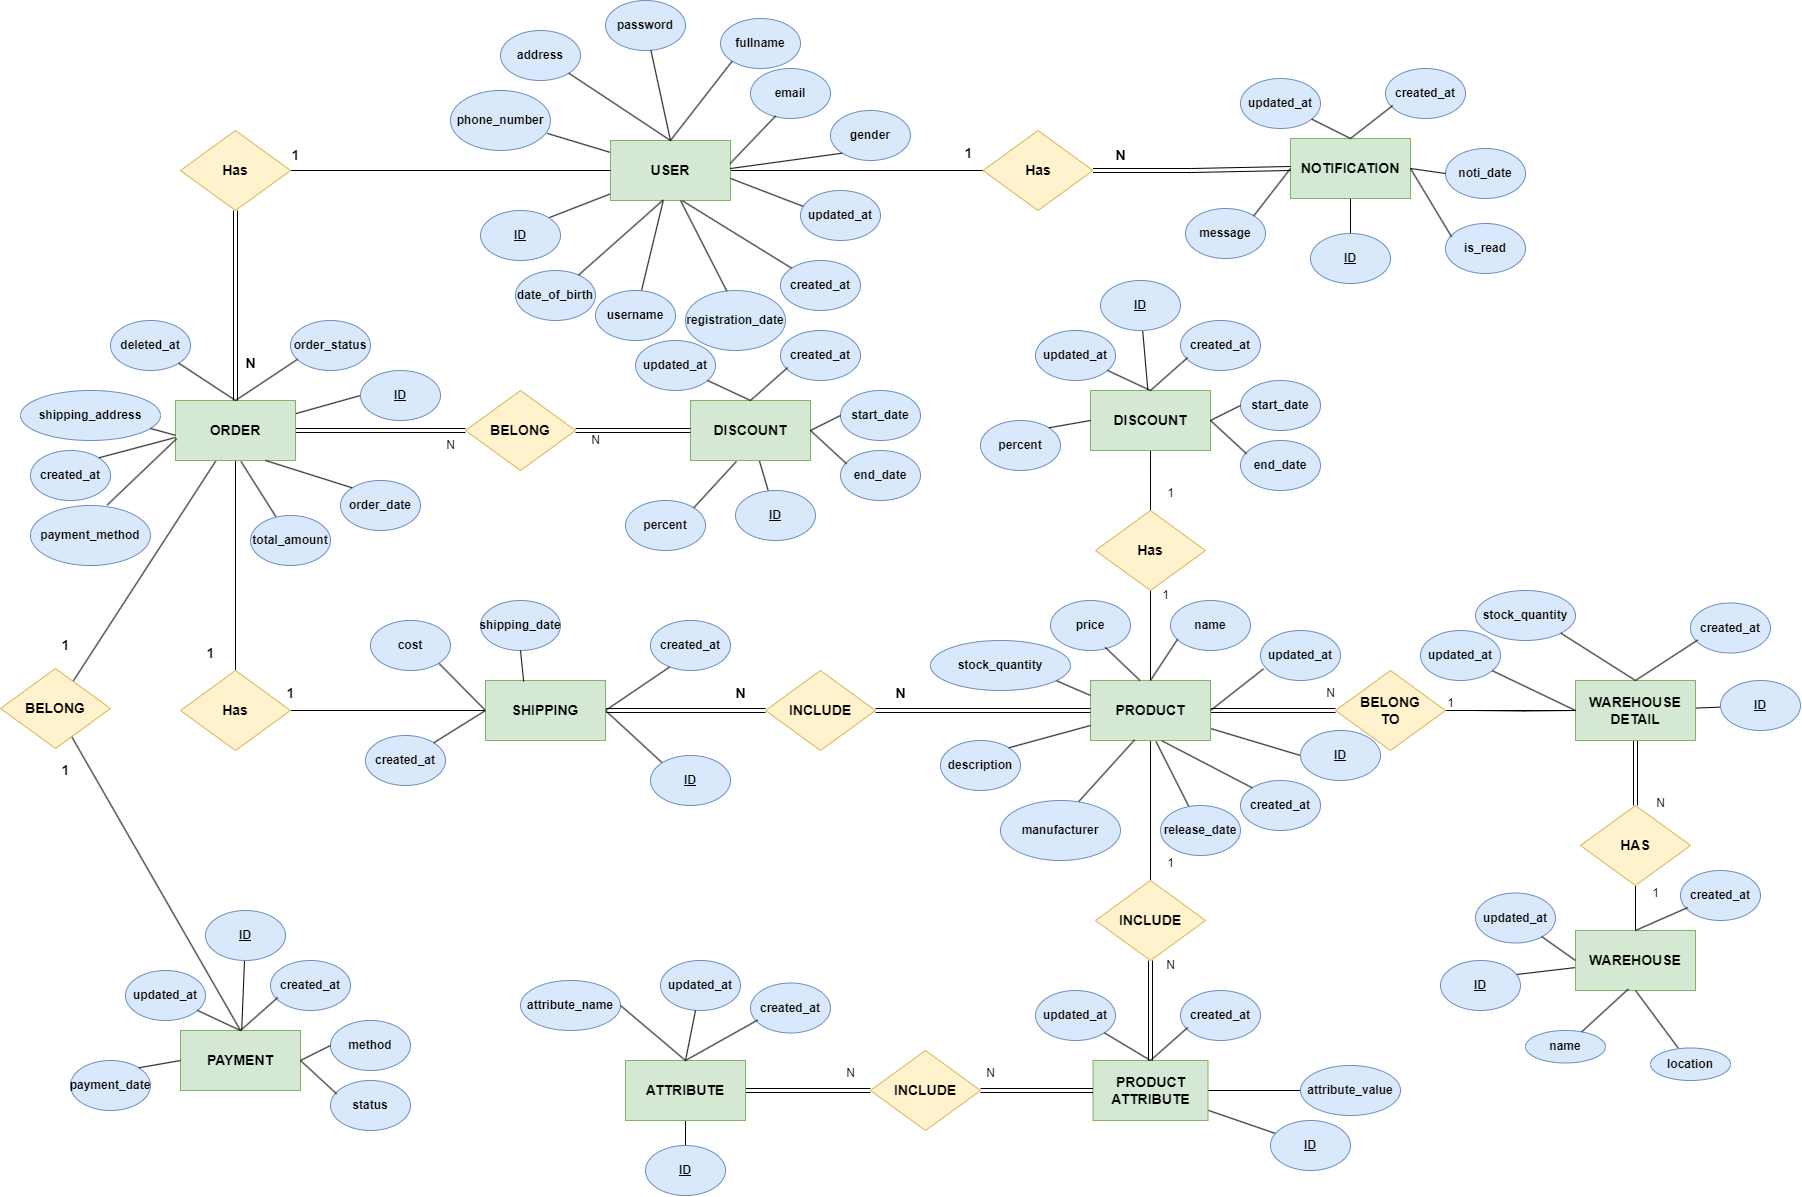
\includegraphics[scale=0.2]{images/hieu/chap-3/database-diagram-dukien.png}
    \caption{Entity Relationship Diagram - Dự kiến}
\end{figure}
\begin{figure}[H]
    \centering
    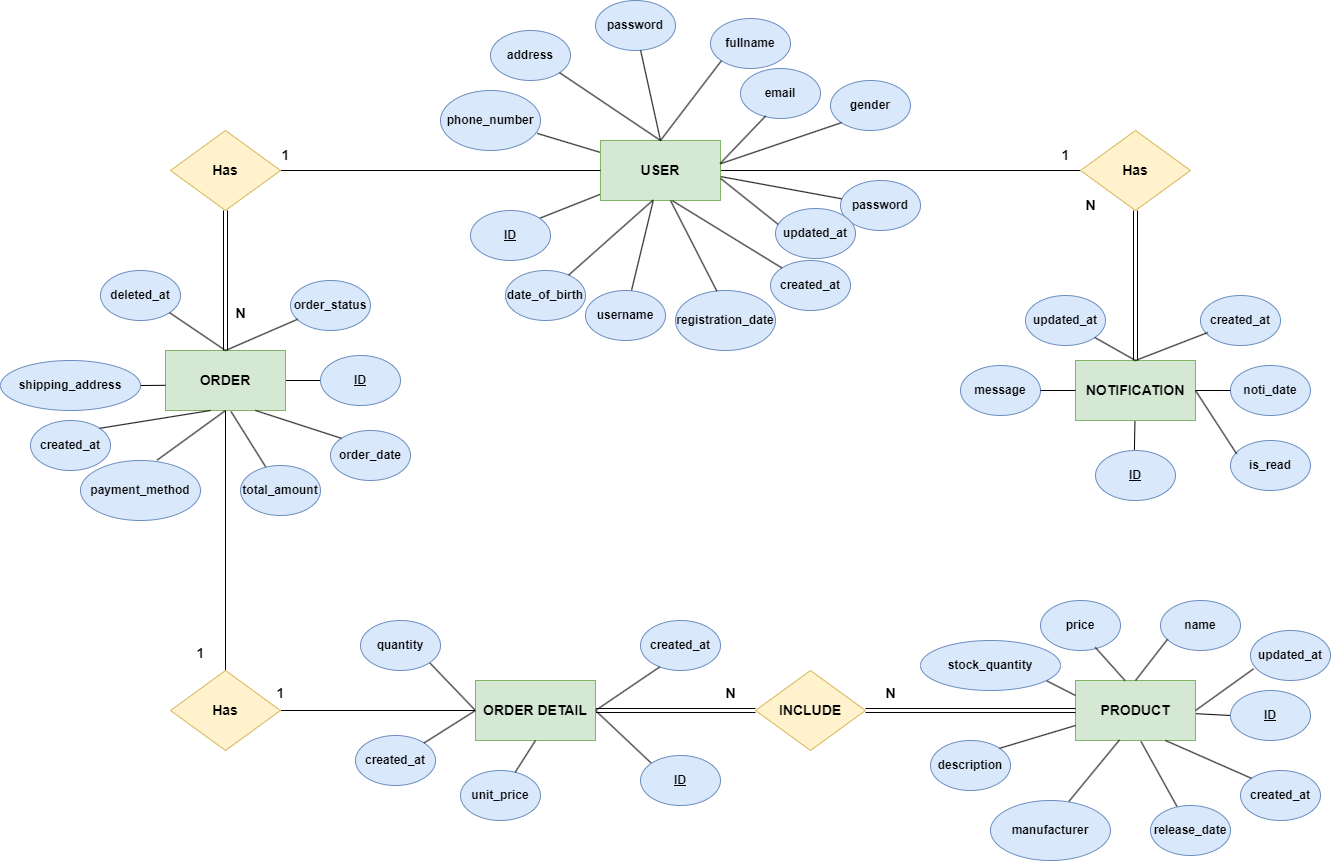
\includegraphics[scale=0.3]{images/hieu/chap-3/full-database-diagram.png}
    \caption{Entity Relationship Diagram - Thực tế}
\end{figure}
\subsubsection {Mô tả chi tiết thực thể}
\begin{itemize}
    \item \textbf{Product:} Thực thể này lưu trữ thông tin về sản phẩm của cửa hàng
        \begin{table}[H]
        \begin{tabular}{|p{3cm}|p{3cm}|p{8cm}|}
        \hline
        \textbf{Thuộc tính} & \textbf{Kiểu dữ liệu} & \textbf{Mô tả}                            \\ \hline
        ID                  & int                   & Mã sản phẩm - khoá chính                  \\ \hline
        name                & varchar               & Tên sản phẩm                              \\ \hline
        desc                & text                  & Mô tả sản phẩm                            \\ \hline
        manufacturer        & varchar               & Nhà sản xuất                              \\ \hline
        release\_date       & date                  & Ngày ra mắt                               \\ \hline
        price               & decimal               & Giá của sản phẩm                          \\ \hline
        stock               & int                   & Số lượng trong kho                        \\ \hline
        created\_at         & timestamp             & Thời gian tạo                             \\ \hline
        updated\_at         & timestamp             & Thời gian cập nhật sản phẩm               \\ \hline
        image\_link         & string                & Liên kết chứa hỉnh ảnh sản phẩm           \\ \hline
        \end{tabular}
        \caption{Bảng mô tả Product}
        \label{table:1}
        \end{table}
    \item \textbf{User:} Thực thể này lưu trữ thông tin về người dùng hệ thống
            \begin{table}[H]
                \begin{tabular}{|p{3cm}|p{3cm}|p{8cm}|}
                \hline
                \textbf{Thuộc tính} & \textbf{Kiểu dữ liệu} & \textbf{Mô tả}                \\ \hline
                ID                  & int                   & Mã người dùng                 \\ \hline
                name                & varchar               & Tên người dùng                \\ \hline
                email               & varchar               & Email người dùng              \\ \hline
                password            & varchar               & Mật khẩu người dùng           \\ \hline
                fullname            & varchar               & Họ và tên người dùng          \\ \hline
                phone               & varchar               & Số điện thoại người dùng      \\ \hline
                address             & varchar               & Địa chỉ người dùng            \\ \hline
                gender              & boolean               & Giới tính người dùng          \\ \hline
                registration\_date  & timestamp             & Ngày đăng ký                  \\ \hline
                date\_of\_birth      & date                  & Ngày sinh người dùng          \\ \hline
                created\_at          & timestamp             & Thời gian tạo                 \\ \hline
                updated\_at          & timestamp             & Thời gian cập nhật            \\ \hline
                \end{tabular}
                \caption{Bảng mô tả User}
                \label{table:2}
                \end{table}
    \item \textbf{Order:} Thực thể này lưu trữ thông tin các đơn hàng người dùng đã đặt
        \begin{table}[H]
            \begin{tabular}{|p{3cm}|p{3cm}|p{8cm}|}
            \hline
            \textbf{Thuộc tính} & \textbf{Kiểu dữ liệu} & \textbf{Mô tả}                \\ \hline
                ID                  & int                   & Mã đơn hàng                   \\ \hline
                order\_date         & timestamp             & Ngày đặt hàng                 \\ \hline
                total\_amount       & decimal               & Tổng số tiền                  \\ \hline
                order\_status       & varchar               & Trạng thái đơn hàng           \\ \hline
                payment\_method     & varchar               & Phương thức thanh toán        \\ \hline
                shipping\_address   & varchar               & Địa chỉ giao hàng             \\ \hline
                created\_at         & timestamp             & Thời gian tạo                 \\ \hline
                updated\_at         & timestamp             & Thời gian cập nhật            \\ \hline
                \end{tabular}
                \caption{Bảng mô tả Order}
                \label{table:3}
        \end{table}
    \item \textbf{Order Detail:} Thực thể này lưu trữ thông tin chi tiết của từng sản phẩm trong đơn hàng
        \begin{table}[H]
        \begin{tabular}{|p{3cm}|p{3cm}|p{8cm}|}
        \hline
        \textbf{Thuộc tính} & \textbf{Kiểu dữ liệu} & \textbf{Mô tả}           \\ \hline
        ID                  & int                   & Mã đơn hàng    \\ \hline
        quantity            & int                   & Số lượng       \\ \hline
        unit\_price         & decimal               & Đơn giá        \\ \hline
        shipping\_fee       & decimal               & Phí vận chuyển \\ \hline
        created\_at         & timestamp             & Thời gian tạo  \\ \hline
        updated\_at         & timestamp             & Thời gian cập nhật \\ \hline
        \end{tabular}
        \caption{Bảng mô tả Order Detail}
        \label{table:4}
        \end{table}
    \item \textbf{Notification:} Đây là một thực thể lưu trữ thông tin về thông báo hệ thống gửi cho người dùng
        \begin{table}[H]
            \begin{tabular}{|p{3cm}|p{3cm}|p{8cm}|}
            \hline
            \textbf{Thuộc tính} & \textbf{Kiểu dữ liệu} & \textbf{Mô tả}         \\ \hline
            ID                  & int                   & Mã thông báo           \\ \hline
            message             & text                  & Nội dung thông báo      \\ \hline
            is\_read            & boolean               & Trạng thái đã đọc      \\ \hline
            noti\_date         & timestamp             & Ngày thông báo         \\ \hline
            created\_at         & timestamp             & Thời gian tạo          \\ \hline
            updated\_at         & timestamp             & Thời gian cập nhật     \\ \hline
            \end{tabular}
            \caption{Bảng mô tả Notification}
        \label{table:5}
        \end{table}
\end{itemize}

\section{Phân tích bài toán và đề xuất giải pháp}

\subsection{Kết luận}
Từ việc phân tích các use case ở chương 2, chúng ta có thể rút ra được một số kết luận như sau:\\[0.5cm]
\noindent Tất cả các use case đều sử dụng nền tảng cloud để xây dựng hệ thống nhằm đáp ứng tính 
scalability (khả năng mở rộng) và availability (tính sẵn sàng). Một số dịch vụ nền tảng cloud phổ biến nhất hiện nay để quản lý Kubernetes là EKS (Elastic Kubernetes Service) và AKS (Azure Kubernetes Service), các dịch vụ này có thể tự động hóa nhiều công việc và tích hợp tốt với các dịch vụ khác trong hệ sinh thái của nhà cung cấp đó nhằm giúp đơn giản hóa việc triển khai và quản lý cụm Kubernetes. \\[0.5cm]
Tuy nhiên, chúng ta có thể sử dụng Kubernetes để triển khai ứng dụng của mình trên bất kỳ nơi nào có hỗ trợ Kubernetes, mà không bị ràng buộc bởi một nhà cung cấp dịch vụ nào, hay nói cách khác nó độc lập với hạ tầng cụ thể. \\[0.5cm]
Bên cạnh đó, Kubernetes còn đảm bảo được hệ thống sẽ đáp ứng được tính scalability (khả năng mở rộng) và availability (tính sẵn sàng) thông qua một số dịch vụ và khái niệm của nó như:
\begin{itemize}
    \item ReplicaSets: Dùng để định nghĩa và duy trì một số lượng replicas (bản sao) của các pod chạy ứng dụng. Điều này giúp đảm bảo tính sẵn sàng của ứng dụng và có thể mở rộng hoặc thu hẹp số lượng replicas dựa trên tải công việc.
    \item Horizontal Pod Autoscaler (HPA): Cho phép tự động thay đổi số lượng replicas của một pod dựa trên các điều kiện như CPU và/hoặc bộ nhớ sử dụng.
    \item Cluster Autoscaler: Tự động mở rộng hoặc thu hẹp cụm Kubernetes bằng cách thêm hoặc giảm số lượng node dựa trên tải công việc.
    \item Load Balancer Services: Sử dụng để phân phối các yêu cầu đến các pod trong cụm, giúp đảm bảo tính sẵn sàng và chia tải đều.
    \item Readiness Probes: Cho phép Kubernetes kiểm tra tính sẵn sàng của mỗi pod trước khi chuyển lưu lượng truy cập đến nó.
    \item Liveness Probes: Kiểm tra xem một pod có hoạt động đúng cách hay không và tự động khởi động lại pod nếu cần.
    \item Pod Disruption Budgets: Giới hạn số lượng pods có thể bị tắt đồng thời trong khi thực hiện các cập nhật hoặc bảo trì để đảm bảo tính sẵn sàng.
\end{itemize}
\noindent Đa phần kiến trúc microservice được ưu tiên áp dụng vì đây là một mô hình ít phụ thuộc vào nhau nên chúng có thể được triển khai, quản lý và mở rộng độc lập với nhau, đồng thời cũng giảm áp lực cho hệ thống vì chúng không cần phải tương tác trực tiếp với nhau mà thông qua message queue (Apache Kafka, RabbitMQ, ActiveMQ, và Microsoft Azure Service Bus).
\subsection{Đề xuất giải pháp}
\noindent Từ các phân tích và kết luận ở trên, nhóm quyết định sẽ xây dựng hệ thống dưới dạng microservice và deloy ứng dụng bằng Kubernetes. Với Kubernetes, ứng dụng sẽ đáp ứng được tính mở rộng và tính sẵn sàng cao thông qua một số dịch vụ mà Kubernetes cung cấp: deloyment, HPA, masternode v.v. Các service của hệ thống sẽ giao tiếp với nhau thông qua message queue.
